%%%%%%%%%%%%%%%%%%%%%%%%%%%%%%%%%%%%%%%%%%%%%%%%%%%%%%%%%%%%%%%%%%%%%%%%%%%%%%%%%%%%%%%%%%%%%%%%%%%%
% NN diagram
% Adapted from: http://www.texample.net/tikz/examples/neural-network/

\RequirePackage{luatex85}
\documentclass[border=0.5mm]{standalone}
\usepackage[a-1b]{pdfx}
\usepackage{tikz}

\usepackage{xcolor}
% Colors from https://styleguide.duke.edu/color-palette/

% These are the official colors, and they cannot be modified by the program (ie changing the opacity or saturation)
\definecolor{Duke Blue}{HTML}{001A57}
\definecolor{Blue Devil Blue}{HTML}{0736A4}

% These are the official recommendations for colors to go with the two official Duke colors. PMS is the Pantone Matching system index, so you can search the color to see what it should look like
\definecolor{PMS Black 3}{HTML}{262626}
\definecolor{PMS Cool Gray 11}{HTML}{666666}
\definecolor{PMS Cool Gray 7}{HTML}{B5B5B5}
\definecolor{PMS Cool Gray 3}{HTML}{E5E5E5}
\definecolor{Light Gray}{HTML}{F5F5F5}

% Blues
\definecolor{PMS 294}{HTML}{003366}
\definecolor{PMS 3015}{HTML}{235F9C}
\definecolor{PMS 3005}{HTML}{0680CD}

% Oranges
\definecolor{PMS 166}{HTML}{D75404}
\definecolor{PMS 1805}{HTML}{CC3300}
% \definecolor{PMS 157}{HTML}{F09905}

% Other
\definecolor{PMS 392}{HTML}{728302} % dark green
\definecolor{PMS 390}{HTML}{A1B70D} % light green
\definecolor{PMS 123}{HTML}{FFD960} % light yellow
\definecolor{PMS 2617}{HTML}{993399} % nice violet


\begin{document}
\resizebox{15cm}{!}{%
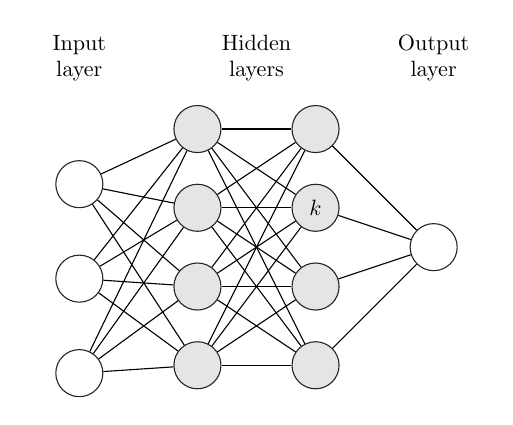
\begin{tikzpicture}[x=1.2cm, y=1.2cm]
  \pgfmathsetmacro{\textscale}{0.8}

  \tikzstyle{annot} = [scale=\textscale,text width=4em, text centered]
  \tikzstyle{neuron}=[circle,draw=PMS Black 3,minimum size=17pt,inner sep=0pt]
  \tikzstyle{hidden neuron}=[neuron, fill=PMS Cool Gray 3];

  % Draw the input layer nodes
  \foreach \y in {1,...,3}
      \node[neuron] (I-\y) at (0,-\y) {};

  % Draw the hidden layer nodes
  \foreach \y in {1,...,4}
      \path[yshift=0.5cm]
          node[hidden neuron] (H1-\y) at (1.5cm,-\y cm) {};

  \foreach \y in {1,...,4}
      \path[yshift=0.5cm]
          node[hidden neuron] (H2-\y) at (3cm,-\y cm) {};

  % Draw the output layer node
  % \node[neuron] (O) at (4.5cm,-2.5cm) {};
  \path[yshift=0.5cm]
      node[neuron] (O) at (4.5cm,-2.5cm) {};

  % Connect every node in the input layer with every node in the hidden layer.
  \foreach \source in {1,...,3}
      \foreach \dest in {1,...,4}
          \path (I-\source) edge (H1-\dest);

  \foreach \source in {1,...,4}
      \foreach \dest in {1,...,4}
          \path (H1-\source) edge (H2-\dest);

  % Connect every node in the hidden layer with the output layer
  \foreach \source in {1,...,4}
      \path (H2-\source) edge (O);

  % Annotate the layers
  \node[above of=H1-1, node distance=0.9cm] (top) {}; % find a good top line
  \node (center) at (2.25cm, 0cm) {}; % 1.5+ 0.75 = 2.25

  % Draw at x |- y coordinate
  \node[annot] at (I-1 |- top) {Input layer};
  \node[annot] at (center |- top) {Hidden layers};
  \node[annot] at (O |- top) {Output layer};

  \node[annot] at (H2-2) {$k$}; % Tie in with neuron diagram

\end{tikzpicture}
} % end resizebox
\end{document}
